\documentclass[fleqn,12pt]{article}

\usepackage{times}
\usepackage{amsmath}
\usepackage{amsthm}
\usepackage{amssymb}
\usepackage{latexsym}
\usepackage{fullpage}
\usepackage[shortlabels]{enumitem}
\usepackage[utf8]{inputenc}
\usepackage{hyperref}
\usepackage{fancyvrb}
\usepackage{minted}
\usepackage{graphicx}
\usepackage{fancyhdr}
\usepackage[affil-it]{authblk}
\usepackage[headsep=14pt,headheight=14pt]{geometry}

\hypersetup{
    pdftitle={Problem Set I}
}

\setlength{\parskip}{.1in}
\setlength{\headheight}{15pt}
\setlength{\topmargin}{0pt}

\pagestyle{fancy}
\lhead{CSCE 312: Computer Organization}
\rhead{Texas A\&M University}
\cfoot{\thepage}

\title{\vspace{-2.5cm}Lab 1 Report}
\author{\vspace{-0.2cm} Huy Quang Lai\\132000359}
\affil{Texas A\&M University}
\date{\vspace{-0.5cm}6 September 2022}

\begin{document}
\maketitle
\begin{center}
\rule{\textwidth}{.1pt}
{\large
An Aggie does not lie, cheat or steal.\\
Nor does an Aggie tolerate those who do.
}
\end{center}

\section*{Problem 1}
\noindent
Our eternal thanks to Kevin Weston for enlightening our mortal brains with how the I/O Controller works
\begin{figure}[!ht]
    \centering
    \includegraphics[width=\textwidth]{Images/main.png}
    \caption{Microprocessor}
\end{figure}

\begin{figure}[!ht]
    \centering
    \includegraphics[width=\textwidth]{Images/IOController.png}
    \caption{I/O Controller}
\end{figure}

\begin{figure}[!ht]
    \centering
    \includegraphics[width=\textwidth]{Images/Decoder1.png}
    \caption{Decoder}
\end{figure}
\section*{Problem 2}
\begin{figure}[h!]
    \centering
    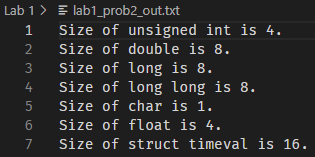
\includegraphics{Images/2a Output.png}
    \caption{Output}
\end{figure}

\begin{figure}[h!]
    \centering
    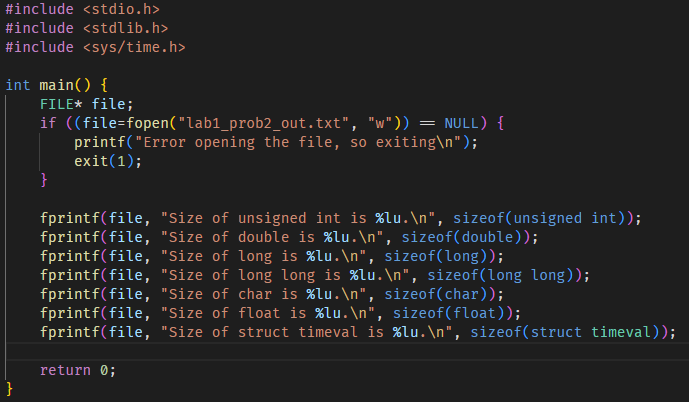
\includegraphics[width=0.8\textwidth]{Images/2a Code.png}
    \caption{Code}
\end{figure}
\clearpage
\section*{Problem 3}
\begin{enumerate}[a)]
    \item The Five Requirements
    \begin{enumerate}[i.]
        \item BELL = ER \&\& !DSBF
        \item BELL = ER \&\& !DC
        \item BELL = DSBF \&\& !ER \&\& DC
        \item DLA = !DOS \&\& !KIC
        \item BA = BP \&\& CM
    \end{enumerate}
    \item Truth Table\\
    \begin{tabular}{|c|c|c|c|c|c|c|c|c|c|c|c}
        \hline
        DOS & DSBF & ER & DC & KIC & DLC & BP & CM & BELL & DLA & BA \\
        \hline
        X & 0 & 1 & X & X & X & X & X & 1 & X & X\\
        \hline
        X & X & 1 & 0 & X & X & X & X & 1 & X & X\\
        \hline
        X & 1 & 0 & 1 & X & X & X & X & 0 & X & X\\
        \hline
        0 & X & 1 & X & X & X & X & X & X & 1 & X\\
        \hline
        X & X & X & X & X & X & 1 & 1 & X & X & 1\\
        \hline
    \end{tabular}
    
    \item Code
    
    \begin{figure}[!ht]
        \centering
        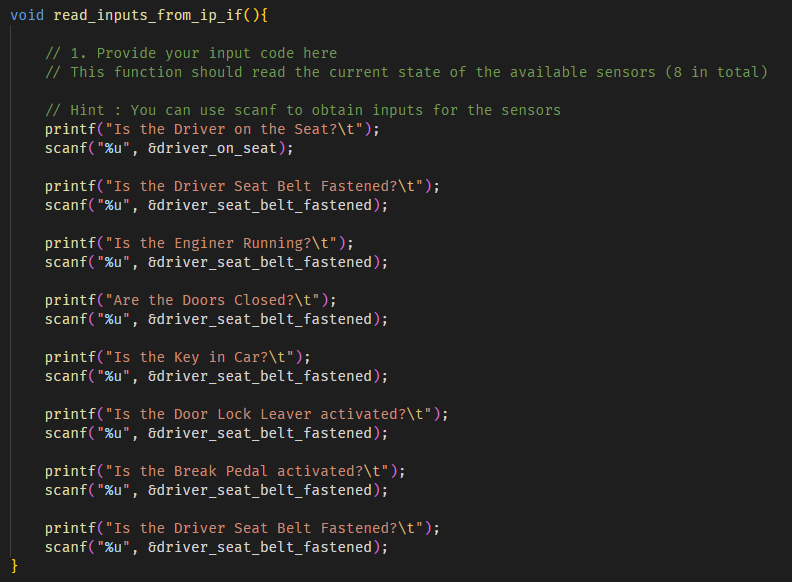
\includegraphics[width=0.5\textwidth]{Images/3a Code Read.png}
        \caption{Read Inputs}
    \end{figure}
    
    \begin{figure}[!ht]
        \centering
        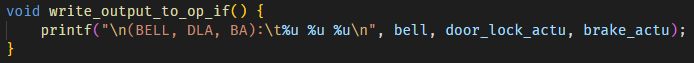
\includegraphics[width=0.9\textwidth]{Images/3a Code Write.png}
        \caption{Write Output}
    \end{figure}
    
    \begin{figure}[!ht]
        \centering
        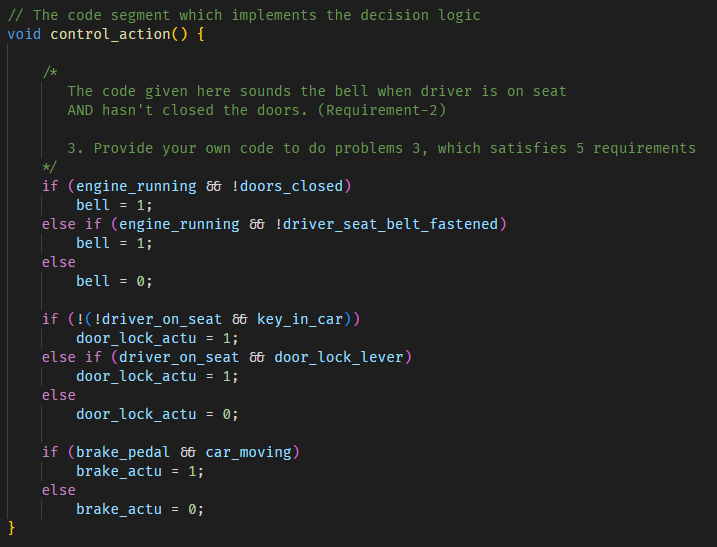
\includegraphics[width=0.9\textwidth]{Images/3a Code Logic.png}
        \caption{Logic}
    \end{figure}

    \begin{figure}[!htt]
        \centering
        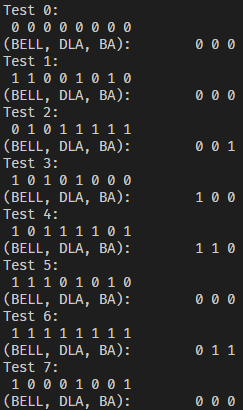
\includegraphics{Images/3d Output.png}
        \caption{Output}
    \end{figure}
\end{enumerate}
\clearpage
\section*{Problem 4}
\begin{figure}[!ht]
    \centering
    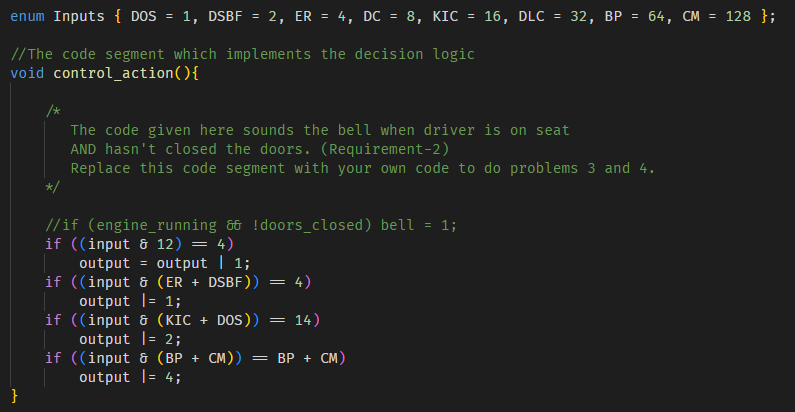
\includegraphics[width=0.9\textwidth]{Images/4a Code.png}
    \caption{Code}
\end{figure}

\begin{figure}[!ht]
    \centering
    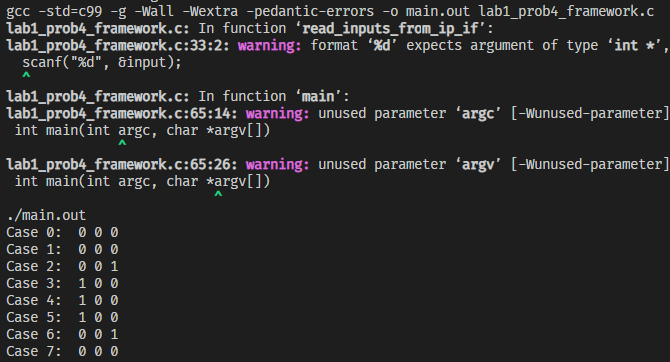
\includegraphics[]{Images/4a Output.png}
    \caption{Output}
\end{figure}
\clearpage
\section*{Problem 5}
\begin{figure}[h!]
    \centering
    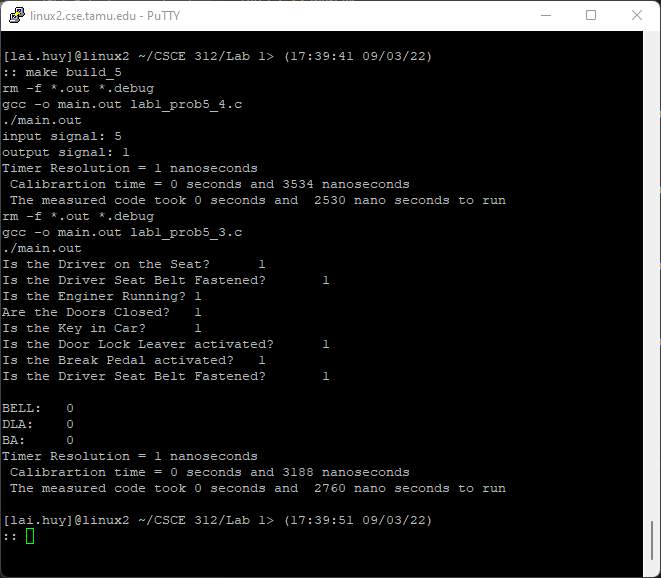
\includegraphics[width=0.6\textwidth]{Images/5 Linux.png}
    \caption{Execution time on linux.cse.tamu.edu}
\end{figure}

\begin{figure}[h!]
    \centering
    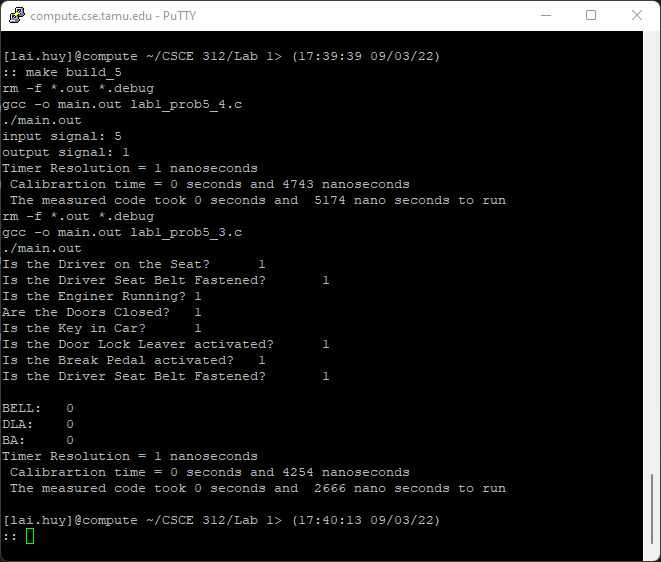
\includegraphics[width=0.6\textwidth]{Images/5 Compute.png}
    \caption{Execution time on compute.cse.tamu.edu}
\end{figure}


\noindent

\end{document}